%!TEX root = main.tex

\section*{Introduction}

Genetic markers have long been used in the 
management of Pacific salmon, and salmon conservation and management has been
a driving force behind a number of advances in molecular ecology,
from data generation techniques \citep{clemento2011discovery,campbell2015genotyping,mckinney2017managing}
to statistical methodology
\citep{smouse1990genetic,anderson2002model,pella2006gibbs}.
Two broadly applicable innovations that have been
actively fostered by the Pacific salmon research community are genetic
stock identification
(GSI:~\citealt{milner1982genetic,beacham2004dna,seeb2007development})
and parentage based tagging
(PBT:~\citealt{anderson2006power, garza2007large, abadia2013large, steele2013validation}).  



 In the 1980's, electrophoretically
detectable genetic variation, in the form of allozymes
\citep{ayala1972allozymes,allendorf1981use}, was used to
establish a program of GSI for Chinook salmon,
{\em Oncorhynchus tshawytscha} \citep{milner1982genetic}.  Extensive sampling
revealed that these allozyme markers
exhibited different allele frequencies among major stocks of Chinook salmon on the West Coast.
These allele frequency differences make GSI possible, and
\citet{milner1985genetic} soon showed that proportions of stocks in
the Washington state coastal troll fishery could be estimated by GSI.
Since that time, with the development of novel molecular markers, and, now
with increasing capacity to sequence genomic material, the scope and scale of GSI
has expanded considerably.

By using greater numbers of more variable markers than the allozymes available
in the 1980s it is possible to accurately
identify the population of origin of individual fish, rather than simply estimating
aggregated stock proportions.  It is also possible to resolve populations of fish that
are much more closely related than before.  Furthermore, reference data sets with genotypes
from hundreds of populations throughout the range of multiple species of salmon and
other anadromous species
\citep{seeb2007development,gilbey2018microsatellite,barclay2019genetic} now exist, and are routinely used to assign fish caught thousands of
kilometers from their natal streams to their stock of origin. Applications include estimating fishery
composition \citep{satterthwaite2015stock}, providing real-time information for genetics-informed fishery closures \citep{beacham2004dna}, assessing the spatial distribution of different stocks in the
ocean \citep{urawa2009stock} and their temporal distribution in upstream migrations
\citep{hess2014monitoring},  and monitoring  bycatch \citep{hasselman2016genetic} or illegal captures \citep{wilmot1999origins} in marine fisheries.

Although sequencing costs continue to decline, they are high enough
that there remains a tradeoff
between reference baselines that include information from a large number of
populations across a broad scale, and those that have been tailored
to distinguish between closely related populations on a smaller, regional scale.
Because of cost considerations, reference baselines that include populations across a broad 
spatial scale may include only a few populations from each sub-region.  Furthermore,
baselines tailored to a specific region often assemble markers that specifically
show allele frequency differences between the closely related---and hence difficult
to resolve---stocks within the region.  Consequently, regionally targeted baselines typically
outperform broad-scale baselines in resolving populations within the region.

The ascendance over the last decade of parentage based tagging (PBT) as a management
tool for Pacific salmon adds another factor to consider when developing a GSI baseline.
Since the first proposal \citep{anderson2005description} to replace or augment the coded-wire tag
programme \citep{nandor2010overview}
with PBT, it has been noted that one of the major advantages of a genetic program for
PBT is that the genetic markers used for PBT could also be useful for GSI (and
vice versa).  This 

Here, we present a reference baseline for Chinook salmon, targeted to the complex population 
structure within the Central Valley of California. Chinook salmon of the two main river basins---the 
Sacramento and the San Joaquin---within the Central Valley exhibit the greatest run-timing diversity
within the species.  With four recognized ecotypes, delineated primarily on the basis of run timing
(Fall-, Late-Fall-, Winter-, and Spring-run), adult Chinook salmon can be found migrating or residing
in freshwater every month of the year in California. NEED MORE HERE. 


 \section*{Methods}

More verbiage

\subsection*{Population Sampling}

We sampled fish for the reference baselines from 7 locations on the across the two
main tributaries (the Sacramento River and the San Joaquin River) within
California's Central Valley. The baseline also includes samples collected from
one location in the Klamath River, and three rivers of the California coast
Fig.~\ref{fig:map}
%%%%%%%%%%%%%
\begin{figure}
\newcommand{\mapcap}{\footnotesize  A map of sampling locations represented in the reference 
baseline.  The colored circles aside
each location name represent the different run-timing groups of Chinook salmon
included in the collections from the location.  Color codes are as follows: \Wball~=~Winter run,
\LFball{}~=~Late-fall run, \Fball~=~Fall run, \Sball~=~Spring run. Abbreviations used in location names as folows: R. = River; Ck. = Creek; H. = Hatchery; NFH = National Fish Hatchery.}
\begin{center}
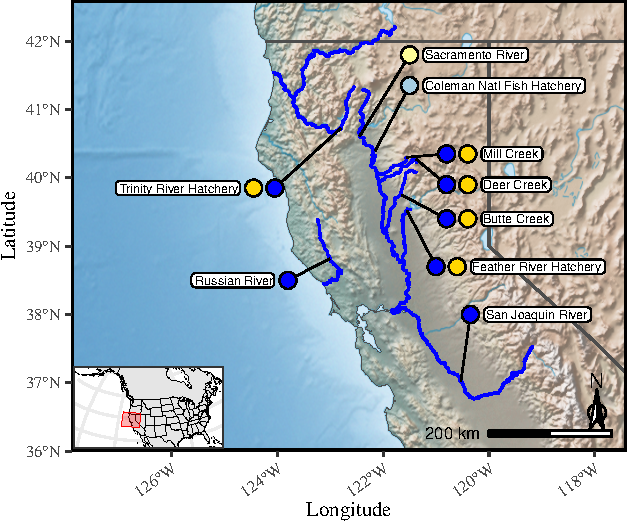
\includegraphics[width=\columnwidth]{images/map-crop.pdf}
\end{center}
\caption[\mapcap]{\mapcap}
\label{fig:map}
\end{figure}
%%%%%%%%%%%%%%%

We are going to stick a table in here:
%%%%%%%%%%%%%%%%
\begin{table*}
\caption{Collections of fish in the reference baseline.  The Sampling Months column shows
a pictorial representation of the proportion of each collection sampled in each month.  Colors in
this column correspond to run-timing groups as described in the caption of Figure~\protect\ref{fig:map}.}
{\small 
\begin{tabular*}{\linewidth}{@{\extracolsep{\fill}} lllllrcr}
\hline\hline\vspace*{0.4ex}
Mainstem River$^1$&Code&Location Name$^2$&Run&Reporting Unit$^4$&ESU$^4$&$N$&$N_\mathrm{day}^5$&Sampling Months&Year Range\tabularnewline
\hline Rogue R.&CRHS&Cole Rivers H.&Spring&SO-NCal-Coast&SONCC&50&0&\raisebox{-0.12 em}{
\includegraphics[height=1.02em]{../tex/images/months-CRHS_Cole-Rivers-Hatchery.pdf}}&2004--2010\tabularnewline
Smith R.&SmRF&Smith R.&Fall&SO-NCal-Coast&SONCC&46&46&\raisebox{-0.12 em}{
\includegraphics[height=1.02em]{../tex/images/months-SmRF_Smith-River.pdf}}&2010--2011\tabularnewline
Klamath R.&BCkF&Blue Ck.&Fall&SO-NCal-Coast&SONCC&56&56&\raisebox{-0.12 em}{
\includegraphics[height=1.02em]{../tex/images/months-BCkF_Blue-Creek.pdf}}&2008--2008\tabularnewline
Klamath R.&IGHF&Iron Gate H.&Fall&Klamath-Trinity&UKTR&93&92&\raisebox{-0.12 em}{
\includegraphics[height=1.02em]{../tex/images/months-IGHF_Iron-Gate-Hatchery.pdf}}&2017--2017\tabularnewline
Trinity R.&TRS&Trinity R. H.&Spring&Klamath-Trinity&UKTR&46&46&\raisebox{-0.12 em}{
\includegraphics[height=1.02em]{../tex/images/months-TRS_Trinity-River-Hatchery.pdf}}&2012--2012\tabularnewline
Trinity R.&TRF&Trinity R. H.&Fall&Klamath-Trinity&UKTR&41&41&\raisebox{-0.12 em}{
\includegraphics[height=1.02em]{../tex/images/months-TRF_Trinity-River-Hatchery.pdf}}&2012--2012\tabularnewline
Eel R.&ERF&Eel R.&Fall&Cent-Cal-Coast&CCC&93&0&\raisebox{-0.12 em}{
\includegraphics[height=1.02em]{../tex/images/months-ERF_Van-Arsdale-Fisheries-Station.pdf}}&2014--2014\tabularnewline
Russian R.&RRF&Warm Springs H.&Fall&Cent-Cal-Coast&CCC&92&92&\raisebox{-0.12 em}{
\includegraphics[height=1.02em]{../tex/images/months-RRF_Warm-Springs-Hatchery.pdf}}&2012--2012\tabularnewline
Sacramento R.&SRW&Livingston Stone NFH&Winter&CV-Winter&CVWR&111&20&\raisebox{-0.12 em}{
\includegraphics[height=1.02em]{../tex/images/months-SRW_Livingston-Stone-National-Fish-Hatchery.pdf}}&2013--2014\tabularnewline
Sacramento R.&BCS&Butte Ck.&Spring&CV-Spring&CVSR&116&116&\raisebox{-0.12 em}{
\includegraphics[height=1.02em]{../tex/images/months-BCS_Butte-Creek.pdf}}&2004--2017\tabularnewline
Sacramento R.&MDS&Deer Ck.&Spring&CV-Spring&CVSR&34&34&\raisebox{-0.12 em}{
\includegraphics[height=1.02em]{../tex/images/months-MDS_Deer-Creek.pdf}}&2002--2002\tabularnewline
Sacramento R.&MDS&Mill Ck.&Spring&CV-Spring&CVSR&50&50&\raisebox{-0.12 em}{
\includegraphics[height=1.02em]{../tex/images/months-MDS_Mill-Creek.pdf}}&2002--2004\tabularnewline
Sacramento R.&FRHS&Feather R. H.&Spring&CV-Fall&CVSR&202&202&\raisebox{-0.12 em}{
\includegraphics[height=1.02em]{../tex/images/months-FRHS_Feather-River-Hatchery.pdf}}&2010--2019\tabularnewline
Sacramento R.&FRHF&Feather R. H.&Fall&CV-Fall&CVFR&106&106&\raisebox{-0.12 em}{
\includegraphics[height=1.02em]{../tex/images/months-FRHF_Feather-River-Hatchery.pdf}}&2008--2010\tabularnewline
Sacramento R.&BCF&Butte Ck.&Fall&CV-Fall&CVFR&45&45&\raisebox{-0.12 em}{
\includegraphics[height=1.02em]{../tex/images/months-BCF_Butte-Creek.pdf}}&2004--2016\tabularnewline
Sacramento R.&MDF&Deer Ck.&Fall&CV-Fall&CVFR&24&24&\raisebox{-0.12 em}{
\includegraphics[height=1.02em]{../tex/images/months-MDF_Deer-Creek.pdf}}&2002--2004\tabularnewline
Sacramento R.&MDF&Mill Ck.&Fall&CV-Fall&CVFR&49&49&\raisebox{-0.12 em}{
\includegraphics[height=1.02em]{../tex/images/months-MDF_Mill-Creek.pdf}}&2002--2004\tabularnewline
San Joaquin R.&SJRF&San Joaquin R.&Fall&CV-Fall&CVFR&79&79&\raisebox{-0.12 em}{
\includegraphics[height=1.02em]{../tex/images/months-SJRF_San-Joaquin-River.pdf}}&2016--2016\tabularnewline
Sacramento R.&CHLF&Coleman NFH&Late-fall&CV-Late-Fall&CVFR&261&261&\raisebox{-0.12 em}{
\includegraphics[height=1.02em]{../tex/images/months-CHLF_Coleman-National-Fish-Hatchery.pdf}}&2011--2015\tabularnewline

\end{tabular*}
}
\rule{3cm}{0.3pt}

{\footnotesize
$^1$R. = River.\\
$^2$Ck. = Creek; NFH = National Fish Hatchery; R. = River; H. = Hatchery.\\
$^3$ESU = Evolutionarily Significant Unit; CVFR = Central Valley Fall Run ESU; CVSR = Central Valley Spring Run ESU; CVWR = 
Central Valley Winter Run ESU; CC = California Coastal ESU; UKTR = Upper Klamath and Trinity Rivers ESU.
}
\hrule\vspace*{0.3ex}\hrule
\end{table*}
%%%%%%%%%%%%%%%%%%%%%

\subsection*{Genetic Markers}

We will say that we took the SNPs from Clemento et al. and made amplicon based
assays of them

Then we must describe the process by which we got more microhaps.

Then we can talk about assays for the subRoSA markers.

Finally we mention that we have a whole section dedicated to finding the LFAR markers.

\subsection*{Identifying and Designing markers from the Late-Fall Associated Region}


\subsection*{Genetic Variation}

\subsection*{Power for genetic stock identification and population assignment}

\subsection*{Power for relationship inference}

\begin{figure}
\newcommand{\examplecap}{\footnotesize Self-assignment rates  ({\bf a)} and pairwise 
$F_\mathrm{ST}$ values ({\bf b)} for the collections in the baseline.  The codes of the populations
appear on the outer margins of the table atop cells colored according to the run-timing group
of the collection.  Interior cells in which the column and row correspond to the same reporting
unit are colored according to the reporting unit.  For self-assignment tallies, the row corresponds
to the true source collection and the column corresponds to the assigned collection. For $F_\mathrm{ST}$ values, the upper triangle was computed using the baseline microhaplotype
data and the lower triangle was calculated with the whole genome sequence data (where available) from \citet{thompson2020complex}}
\begin{center}
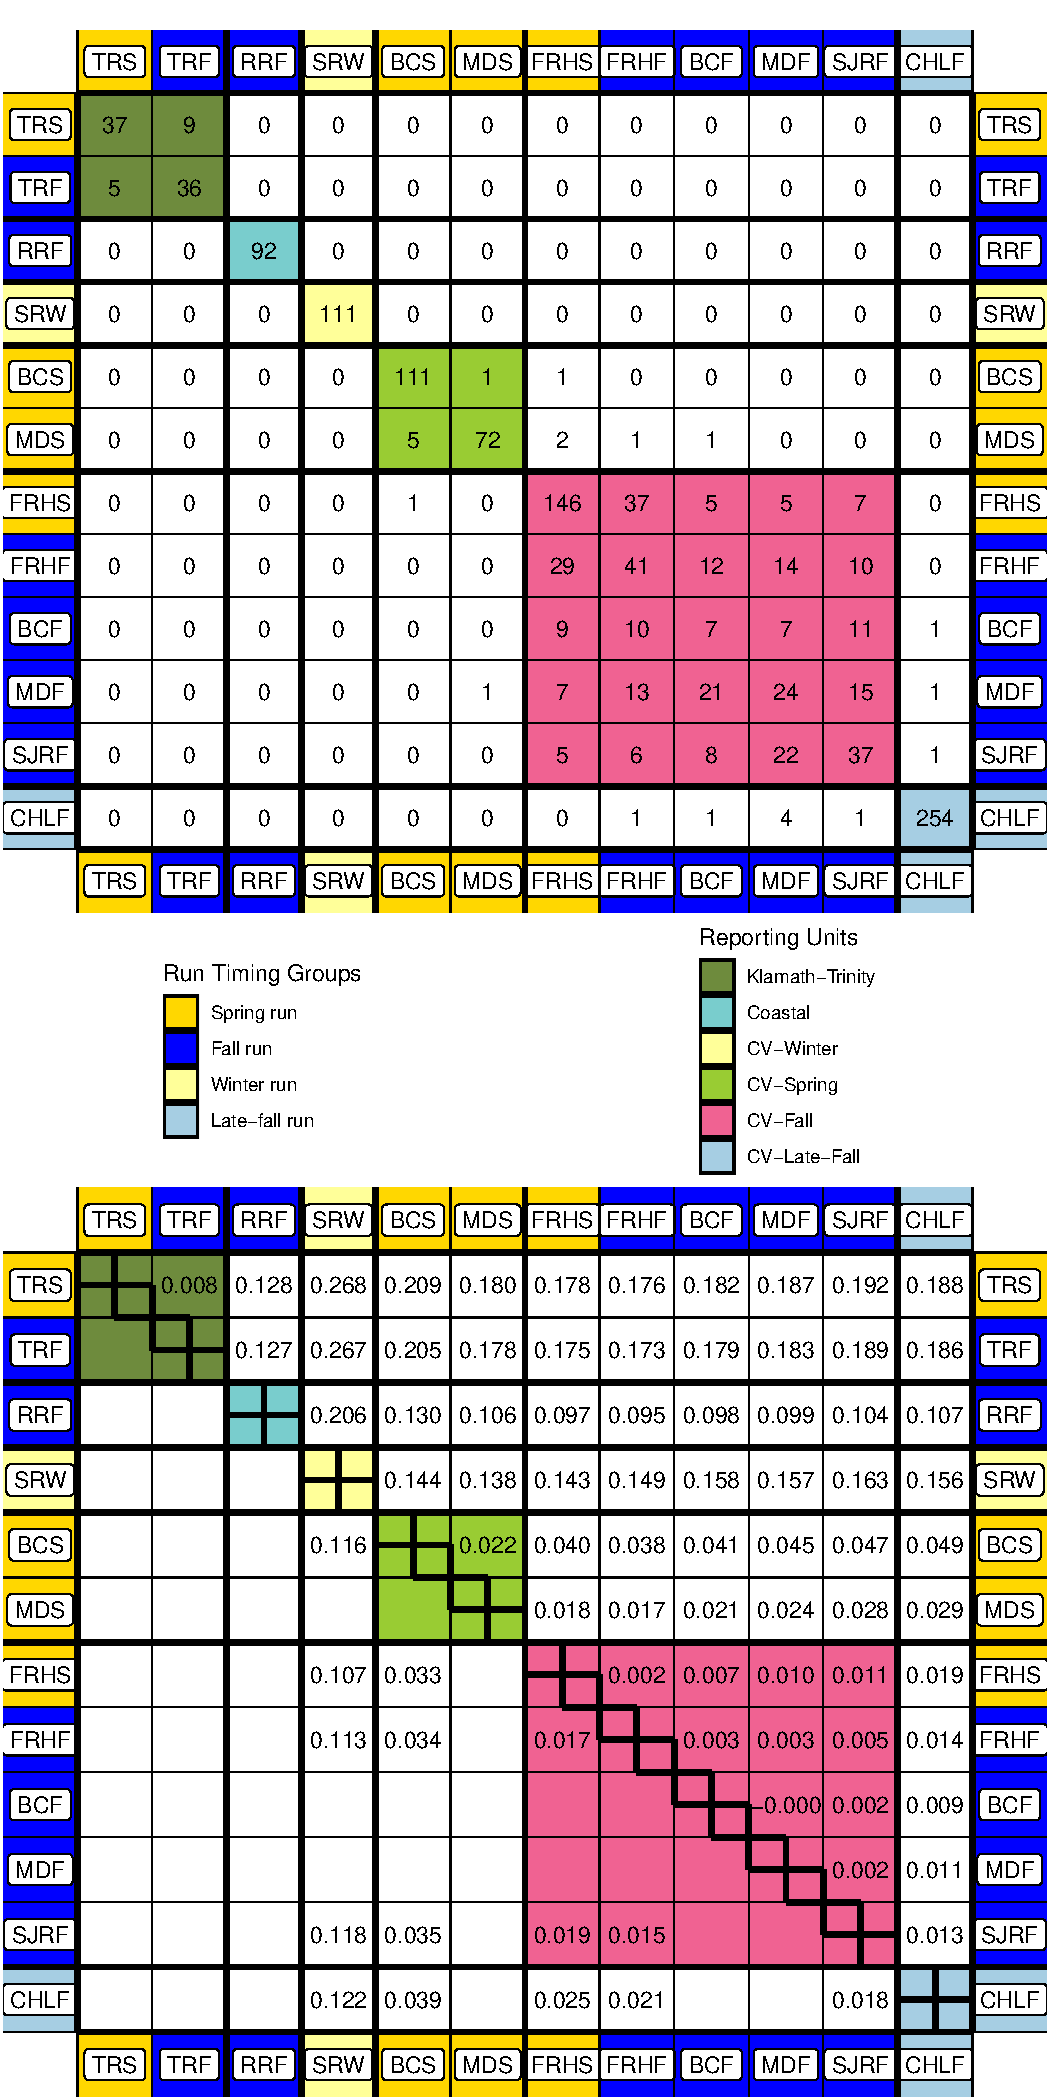
\includegraphics[width=\columnwidth]{images/gsi_and_fst_fig-crop.pdf}
\end{center}
\caption[\examplecap]{\examplecap}
\label{fig:example}
\end{figure}


\section*{Discussion}

When, and if, sequencing costs drop sufficiently, it may  be possible to include
all different populations of a single species within a single standardized reference baseline
that performs equally well at broad and regional scales. A statistical approach for population
assignment from low coverage whole genome sequences appeared recently
\citep{desaixINPRESSpopulation}, and its authors noted that such a data type could
be ideal for producing reference baselines simultaneously applicable to broad scale
coverage and high resolution within sub-regions.   For the present, however,
baselines tailored to specific regions are essential for regional management questions.
It should be noted that recent 

